\documentclass{standalone}
\usepackage{tikz}
\usetikzlibrary{patterns, positioning}


\begin{document}
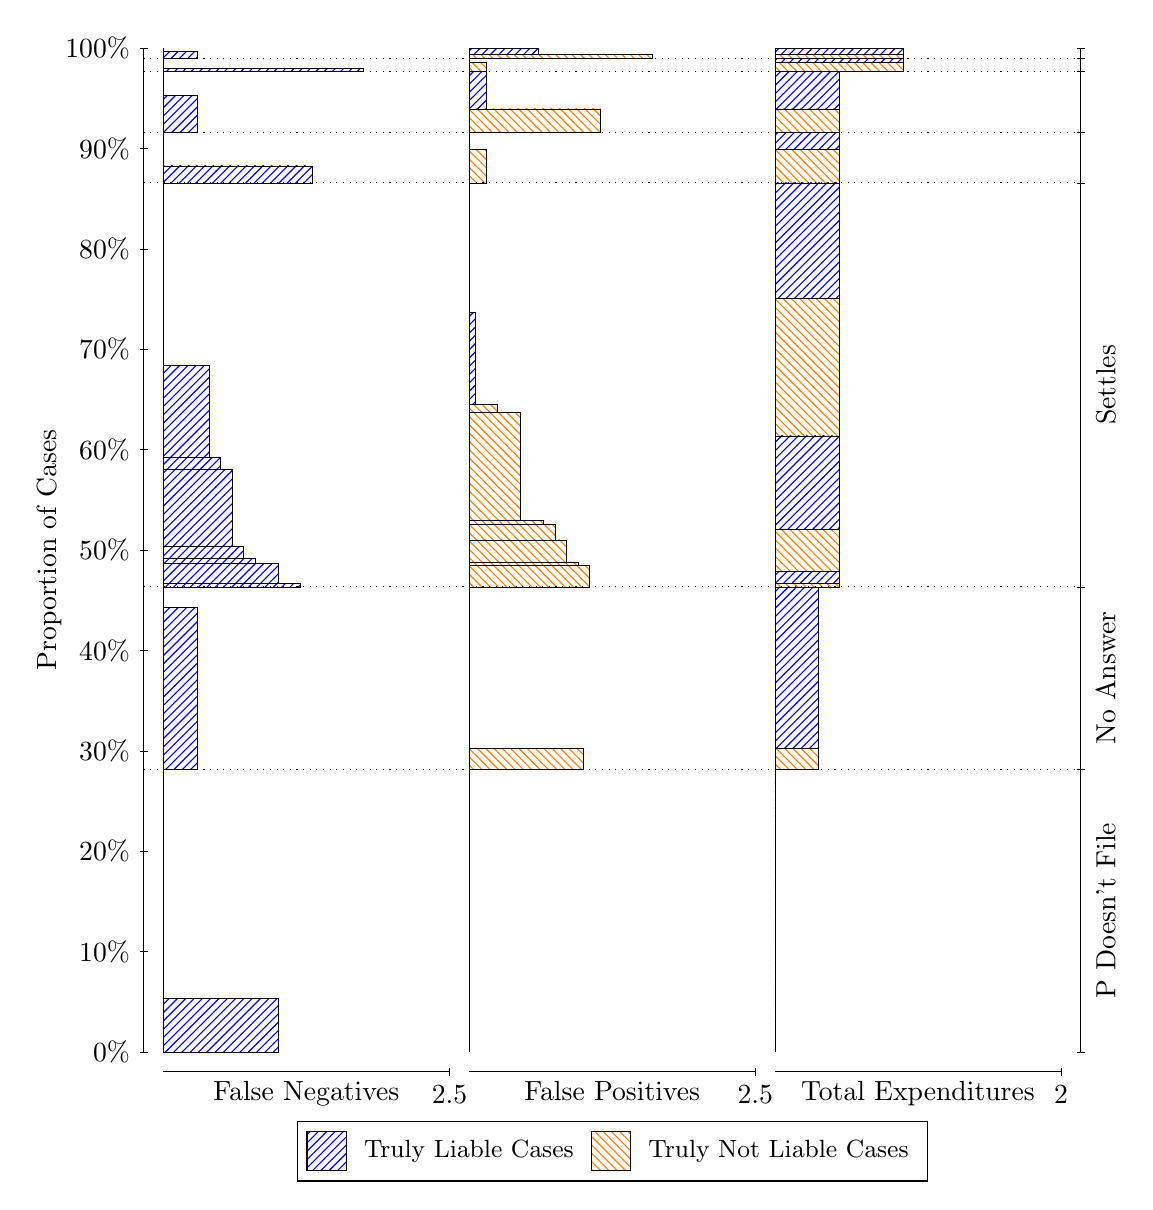
\begin{tikzpicture}
\draw[black, very thin] (1.5,1.75) -- (1.5,14.5);
\node[rotate=90, text=black, anchor=center] at (0.3, 8.125) {Proportion of Cases};
\draw[black, very thin] (1.45,1.75) -- (1.55,1.75);
\node[text=black, anchor=east] at (1.45, 1.75) {0\%};
\draw[black, very thin] (1.45,3.025) -- (1.55,3.025);
\node[text=black, anchor=east] at (1.45, 3.025) {10\%};
\draw[black, very thin] (1.45,4.3) -- (1.55,4.3);
\node[text=black, anchor=east] at (1.45, 4.3) {20\%};
\draw[black, very thin] (1.45,5.575) -- (1.55,5.575);
\node[text=black, anchor=east] at (1.45, 5.575) {30\%};
\draw[black, very thin] (1.45,6.85) -- (1.55,6.85);
\node[text=black, anchor=east] at (1.45, 6.85) {40\%};
\draw[black, very thin] (1.45,8.125) -- (1.55,8.125);
\node[text=black, anchor=east] at (1.45, 8.125) {50\%};
\draw[black, very thin] (1.45,9.4) -- (1.55,9.4);
\node[text=black, anchor=east] at (1.45, 9.4) {60\%};
\draw[black, very thin] (1.45,10.675) -- (1.55,10.675);
\node[text=black, anchor=east] at (1.45, 10.675) {70\%};
\draw[black, very thin] (1.45,11.95) -- (1.55,11.95);
\node[text=black, anchor=east] at (1.45, 11.95) {80\%};
\draw[black, very thin] (1.45,13.225) -- (1.55,13.225);
\node[text=black, anchor=east] at (1.45, 13.225) {90\%};
\draw[black, very thin] (1.45,14.5) -- (1.55,14.5);
\node[text=black, anchor=east] at (1.45, 14.5) {100\%};

\draw[black, very thin] (13.4,1.75) -- (13.4,14.5);
\draw[black, very thin] (13.35,1.75) -- (13.45,1.75);
\node[anchor=west] at (13.35, 1.75) {};
\draw[black, very thin] (13.35,5.3399) -- (13.45,5.3399);
\node[anchor=west] at (13.35, 5.3399) {};
\draw[black, very thin] (13.35,7.6559) -- (13.45,7.6559);
\node[anchor=west] at (13.35, 7.6559) {};
\draw[black, very thin] (13.35,12.787) -- (13.45,12.787);
\node[anchor=west] at (13.35, 12.787) {};
\draw[black, very thin] (13.35,13.429) -- (13.45,13.429);
\node[anchor=west] at (13.35, 13.429) {};
\draw[black, very thin] (13.35,14.199) -- (13.45,14.199);
\node[anchor=west] at (13.35, 14.199) {};
\draw[black, very thin] (13.35,14.368) -- (13.45,14.368);
\node[anchor=west] at (13.35, 14.368) {};
\draw[black, very thin] (13.35,14.5) -- (13.45,14.5);
\node[anchor=west] at (13.35, 14.5) {};

\draw[black, very thin, pattern color=blue, pattern=north east lines] (1.75,1.75) rectangle (3.2033,2.4344);
\draw[black, very thin, pattern color=orange, pattern=north west lines] (1.75,2.4344) rectangle (1.75,5.3399);
\draw[black, very thin, pattern color=blue, pattern=north east lines] (1.75,5.3399) rectangle (2.186,7.3943);
\draw[black, very thin, pattern color=orange, pattern=north west lines] (1.75,7.3943) rectangle (1.75,7.6559);
\draw[black, very thin, pattern color=blue, pattern=north east lines] (1.75,7.6559) rectangle (3.494,7.7022);
\draw[black, very thin, pattern color=blue, pattern=north east lines] (1.75,7.7022) rectangle (3.2033,7.9529);
\draw[black, very thin, pattern color=blue, pattern=north east lines] (1.75,7.9529) rectangle (3.058,7.9565);
\draw[black, very thin, pattern color=blue, pattern=north east lines] (1.75,7.9565) rectangle (2.9127,8.0186);
\draw[black, very thin, pattern color=blue, pattern=north east lines] (1.75,8.0186) rectangle (2.7673,8.1738);
\draw[black, very thin, pattern color=blue, pattern=north east lines] (1.75,8.1738) rectangle (2.622,9.1458);
\draw[black, very thin, pattern color=blue, pattern=north east lines] (1.75,9.1458) rectangle (2.4767,9.304);
\draw[black, very thin, pattern color=blue, pattern=north east lines] (1.75,9.304) rectangle (2.3313,10.471);
\draw[black, very thin, pattern color=orange, pattern=north west lines] (1.75,10.471) rectangle (1.75,12.787);
\draw[black, very thin, pattern color=blue, pattern=north east lines] (1.75,12.787) rectangle (3.6393,13.002);
\draw[black, very thin, pattern color=orange, pattern=north west lines] (1.75,13.002) rectangle (1.75,13.429);
\draw[black, very thin, pattern color=blue, pattern=north east lines] (1.75,13.429) rectangle (2.186,13.902);
\draw[black, very thin, pattern color=orange, pattern=north west lines] (1.75,13.902) rectangle (1.75,14.199);
\draw[black, very thin, pattern color=blue, pattern=north east lines] (1.75,14.199) rectangle (4.2933,14.246);
\draw[black, very thin, pattern color=orange, pattern=north west lines] (1.75,14.246) rectangle (1.75,14.368);
\draw[black, very thin, pattern color=blue, pattern=north east lines] (1.75,14.368) rectangle (2.186,14.453);
\draw[black, very thin, pattern color=orange, pattern=north west lines] (1.75,14.453) rectangle (1.75,14.5);
\draw[black, very thin, pattern color=orange, pattern=north west lines] (5.6333,1.75) rectangle (5.6333,4.6554);
\draw[black, very thin, pattern color=blue, pattern=north east lines] (5.6333,4.6554) rectangle (5.6333,5.3399);
\draw[black, very thin, pattern color=orange, pattern=north west lines] (5.6333,5.3399) rectangle (7.0867,5.6014);
\draw[black, very thin, pattern color=blue, pattern=north east lines] (5.6333,5.6014) rectangle (5.6333,7.6559);
\draw[black, very thin, pattern color=orange, pattern=north west lines] (5.6333,7.6559) rectangle (7.1593,7.927);
\draw[black, very thin, pattern color=orange, pattern=north west lines] (5.6333,7.927) rectangle (7.014,7.9673);
\draw[black, very thin, pattern color=orange, pattern=north west lines] (5.6333,7.9673) rectangle (6.8687,8.2542);
\draw[black, very thin, pattern color=orange, pattern=north west lines] (5.6333,8.2542) rectangle (6.7233,8.4467);
\draw[black, very thin, pattern color=orange, pattern=north west lines] (5.6333,8.4467) rectangle (6.578,8.4987);
\draw[black, very thin, pattern color=orange, pattern=north west lines] (5.6333,8.4987) rectangle (6.4327,8.5023);
\draw[black, very thin, pattern color=orange, pattern=north west lines] (5.6333,8.5023) rectangle (6.2873,9.8687);
\draw[black, very thin, pattern color=orange, pattern=north west lines] (5.6333,9.8687) rectangle (5.9967,9.9718);
\draw[black, very thin, pattern color=blue, pattern=north east lines] (5.6333,9.9718) rectangle (5.706,11.139);
\draw[black, very thin, pattern color=blue, pattern=north east lines] (5.6333,11.139) rectangle (5.6333,12.787);
\draw[black, very thin, pattern color=orange, pattern=north west lines] (5.6333,12.787) rectangle (5.8513,13.214);
\draw[black, very thin, pattern color=blue, pattern=north east lines] (5.6333,13.214) rectangle (5.6333,13.429);
\draw[black, very thin, pattern color=orange, pattern=north west lines] (5.6333,13.429) rectangle (7.3047,13.726);
\draw[black, very thin, pattern color=blue, pattern=north east lines] (5.6333,13.726) rectangle (5.8513,14.199);
\draw[black, very thin, pattern color=orange, pattern=north west lines] (5.6333,14.199) rectangle (5.8513,14.321);
\draw[black, very thin, pattern color=blue, pattern=north east lines] (5.6333,14.321) rectangle (5.6333,14.368);
\draw[black, very thin, pattern color=orange, pattern=north west lines] (5.6333,14.368) rectangle (7.9587,14.415);
\draw[black, very thin, pattern color=blue, pattern=north east lines] (5.6333,14.415) rectangle (6.5053,14.5);
\draw[black, very thin, pattern color=orange, pattern=north west lines] (9.5167,1.75) rectangle (9.5167,4.6554);
\draw[black, very thin, pattern color=blue, pattern=north east lines] (9.5167,4.6554) rectangle (9.5167,5.3399);
\draw[black, very thin, pattern color=orange, pattern=north west lines] (9.5167,5.3399) rectangle (10.062,5.6014);
\draw[black, very thin, pattern color=blue, pattern=north east lines] (9.5167,5.6014) rectangle (10.062,7.6559);
\draw[black, very thin, pattern color=orange, pattern=north west lines] (9.5167,7.6559) rectangle (10.334,7.6961);
\draw[black, very thin, pattern color=blue, pattern=north east lines] (9.5167,7.6961) rectangle (10.334,7.8543);
\draw[black, very thin, pattern color=orange, pattern=north west lines] (9.5167,7.8543) rectangle (10.334,8.3857);
\draw[black, very thin, pattern color=blue, pattern=north east lines] (9.5167,8.3857) rectangle (10.334,9.5751);
\draw[black, very thin, pattern color=orange, pattern=north west lines] (9.5167,9.5751) rectangle (10.334,11.319);
\draw[black, very thin, pattern color=blue, pattern=north east lines] (9.5167,11.319) rectangle (10.334,12.787);
\draw[black, very thin, pattern color=orange, pattern=north west lines] (9.5167,12.787) rectangle (10.334,13.214);
\draw[black, very thin, pattern color=blue, pattern=north east lines] (9.5167,13.214) rectangle (10.334,13.429);
\draw[black, very thin, pattern color=orange, pattern=north west lines] (9.5167,13.429) rectangle (10.334,13.726);
\draw[black, very thin, pattern color=blue, pattern=north east lines] (9.5167,13.726) rectangle (10.334,14.199);
\draw[black, very thin, pattern color=orange, pattern=north west lines] (9.5167,14.199) rectangle (11.152,14.321);
\draw[black, very thin, pattern color=blue, pattern=north east lines] (9.5167,14.321) rectangle (11.152,14.368);
\draw[black, very thin, pattern color=orange, pattern=north west lines] (9.5167,14.368) rectangle (11.152,14.415);
\draw[black, very thin, pattern color=blue, pattern=north east lines] (9.5167,14.415) rectangle (11.152,14.5);
\draw[black, dotted] (1.5,5.3399) -- (13.4,5.3399);
\draw[black, dotted] (1.5,7.6559) -- (13.4,7.6559);
\draw[black, dotted] (1.5,12.787) -- (13.4,12.787);
\draw[black, dotted] (1.5,13.429) -- (13.4,13.429);
\draw[black, dotted] (1.5,14.199) -- (13.4,14.199);
\draw[black, dotted] (1.5,14.368) -- (13.4,14.368);
\draw[black, very thin] (1.75,1.5) -- (5.3833,1.5);
\node[text=black, anchor=north] at (3.5667, 1.5) {False Negatives};
\draw[black, very thin] (5.3833,1.45) -- (5.3833,1.55);
\node[text=black, anchor=north] at (5.3833, 1.45) {2.5};

\draw[black, very thin] (5.6333,1.5) -- (9.2667,1.5);
\node[text=black, anchor=north] at (7.45, 1.5) {False Positives};
\draw[black, very thin] (9.2667,1.45) -- (9.2667,1.55);
\node[text=black, anchor=north] at (9.2667, 1.45) {2.5};

\draw[black, very thin] (9.5167,1.5) -- (13.15,1.5);
\node[text=black, anchor=north] at (11.333, 1.5) {Total Expenditures};
\draw[black, very thin] (13.15,1.45) -- (13.15,1.55);
\node[text=black, anchor=north] at (13.15, 1.45) {2};

\node[text=black, centered, rotate=90] at (13.72, 3.5449) {P Doesn't File};
\node[text=black, centered, rotate=90] at (13.72, 6.4979) {No Answer};
\node[text=black, centered, rotate=90] at (13.72, 10.222) {Settles};





\draw (7.449999999999999,1.5) node[draw=none] (baseCoordinate) {};
\begin{scope}[align=center]
        \matrix[scale=0.5, draw=black, below=0.5cm of baseCoordinate, nodes={draw}, column sep=0.1cm]{
            \node[rectangle, draw, minimum width=0.5cm, minimum height=0.5cm, pattern color=blue, pattern=north east lines] {}; &
            \node[draw=none, font=\small, text=black] (B) {Truly Liable Cases}; &
            \node[rectangle, draw, minimum width=0.5cm, minimum height=0.5cm, pattern color=orange, pattern=north west lines] {}; &
            \node[draw=none, font=\small, text=black] (B) {Truly Not Liable Cases}; \\
            };
\end{scope}

\end{tikzpicture}
\end{document}